\documentclass[a4paper,10pt]{report}
\usepackage[utf8]{inputenc}
\usepackage{graphicx}
\usepackage{verbatim}
\usepackage{ctable} % for \specialrule command

\usepackage[a4paper, total={6in, 8in}]{geometry}
% Title Page
\title{\textbf{OPTICAL COMMUNICATION COMPONENTS \\ Lab 9}}
\author{Nicola Simoni, Tadewos Somano, Melkamsew Tenaw}
\date{University of Brescia, Faculty of Engineering\\A.Y. 2013-2014}


\begin{document}
\maketitle

%%%%%%%%%%%%%%%%%%%%%%%%%%%%%%%%%%%%%%%%%%%%%%%%%%%%%%%%%%%%%%%%%%%%%%%%%%%%%%%%%%%%%%%%%%%%%
\section*{10G-40G Upgrade}

We use a 175 Km unrepeated link with a booster amplifier at the transmitter and a pre-amp at the receiver.
A Raman pump backward pumps the transmission fiber from the receiver terminal end.
We compare the Optical SNR (OSNR) versus frequency for 10 and 40 Gb/s transmissions with both Raman pump turned on and off.
The parameters are the following:
\begin{itemize}
 \item Gain: 100 dB
 \item Noise Figure: 5 dB
 \item Output Power: 0.1 W
\end{itemize}

In Figure \ref{q1a_10} is shown the result for 10 Gb/s and Raman pump turned off,
while in Figure \ref{q1a_10_ramanon} is shown the result for the same bit-rate and Raman pump turned on.
In Figure \ref{q1a_40} is shown the result for 40 Gb/s and Raman pump turned off,
while in Figure \ref{q1a_40_ramanon} is shown the result for the same bit-rate and Raman pump turned on.


\begin{figure}[!ht]
   \centering
   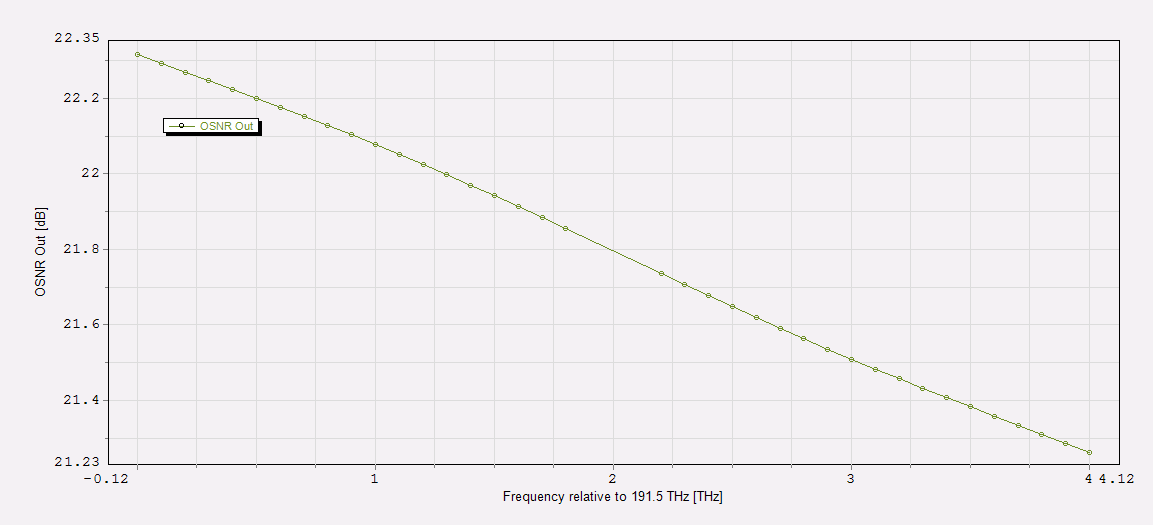
\includegraphics[width=12cm]{q1a_10.png}\\
   \caption{OSNR versus frequency, 10 Gb/s, Raman OFF.}
   \label{q1a_10}
\end{figure}
   
\begin{figure}[!ht]
   \centering
   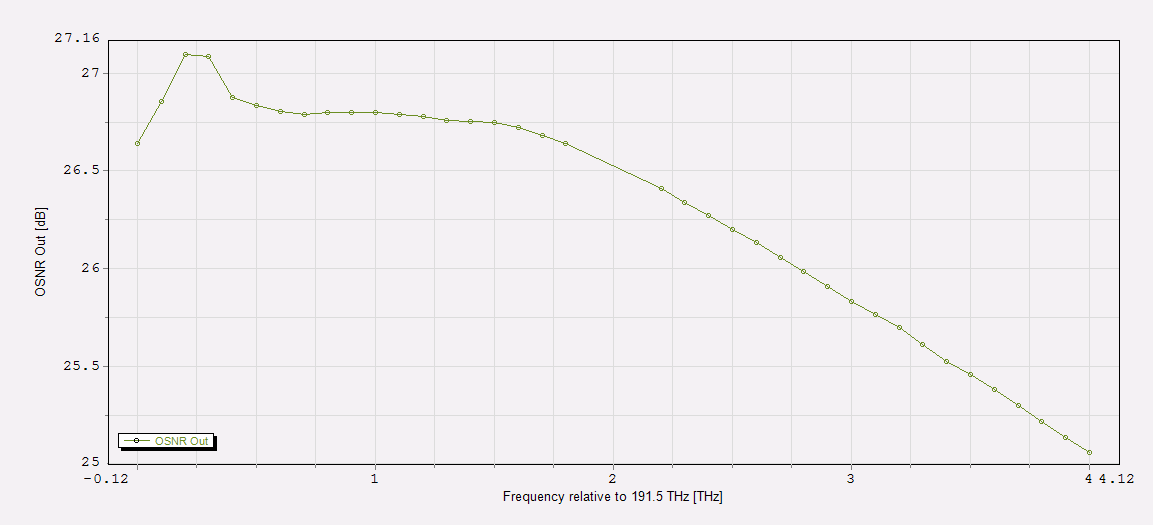
\includegraphics[width=12cm]{q1a_10_ramanon.png}\\
   \caption{OSNR versus frequency, 10 Gb/s, Raman ON.}
   \label{q1a_10_ramanon}
\end{figure}

\begin{figure}[!ht]
   \centering
   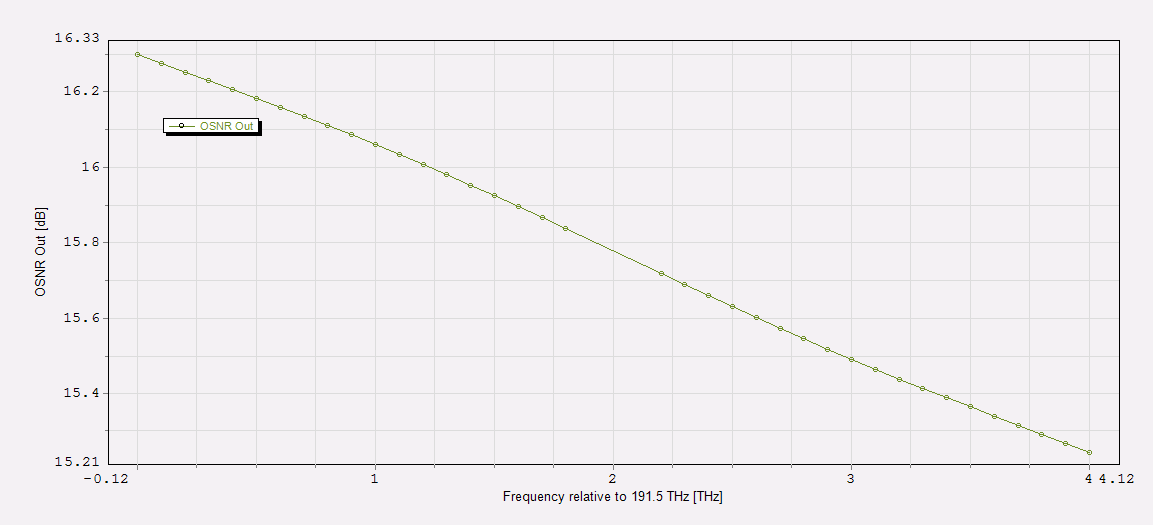
\includegraphics[width=12cm]{q1a_40.png}\\
   \caption{OSNR versus frequency, 40 Gb/s, Raman OFF.}
   \label{q1a_40}
\end{figure}
   
\begin{figure}[!ht]
   \centering
   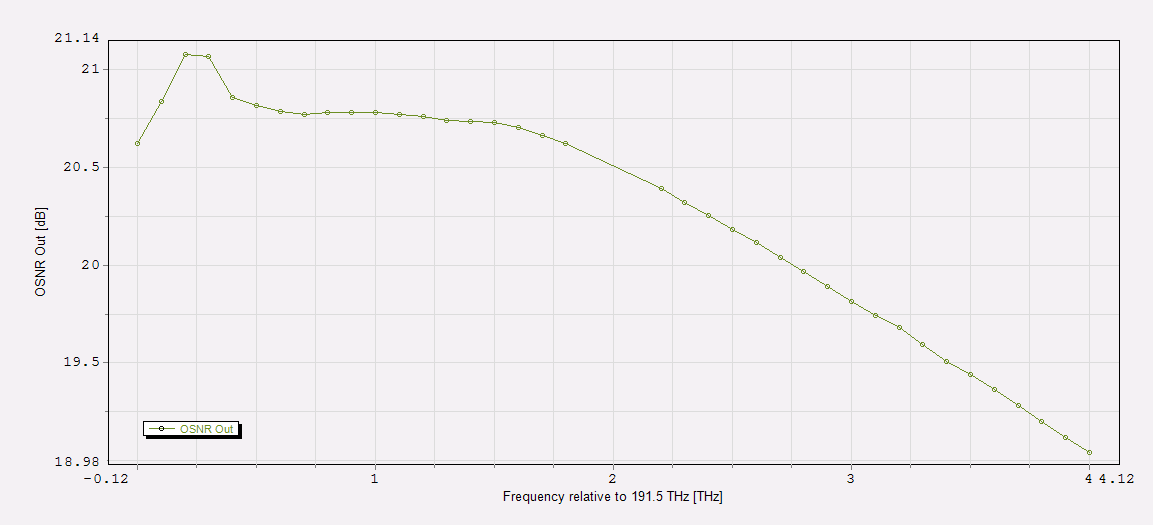
\includegraphics[width=12cm]{q1a_40_ramanon.png}\\
   \caption{OSNR versus frequency, 40 Gb/s, Raman ON.}
   \label{q1a_40_ramanon}
\end{figure}

In Table \ref{ber} are reported the BER values, measured from the eye diagram, for the four cases.
\begin{table}[ht!]
  \begin{center}
    \begin{tabular}{|c|c|c|}
      \specialrule{.1em}{.05em}{.05em}
	 Bitrate [Gb/s] & Raman & BER \\
	\hline
	10 & OFF & $4.975 \cdot 10^{-11}$\\
	\hline
	10 & ON & $1.612 \cdot 10^{-70}$\\
	\hline
	40 & OFF & $1.086 \cdot 10^{-4}$\\
	\hline
	40 & ON & $2.354 \cdot 10^{-27}$\\
      \specialrule{.1em}{.05em}{.05em}
    \end{tabular}
  \end{center}
\caption{BERs.}
\label{ber}
\label{tab}
\end{table}


\newpage
%%%%%%%%%%%%%%%%%%%%%%%%%%%%%%%%%%%%%%%%%%%%%%%%%%%%%%%%%%%%%%%%%%%%%%%%%%%%%%%%%%%%%%%%%%%%%
\subsection*{Question 1A}
By looking at the graphs we can observe that, increasing the bit-rate from 10 to 40 Gb/s,
the OSNR decreases of nearly 6 dB. This happens when the Raman pump is both ON and OFF.

%%%%%%%%%%%%%%%%%%%%%%%%%%%%%%%%%%%%%%%%%%%%%%%%%%%%%%%%%%%%%%%%%%%%%%%%%%%%%%%%%%%%%%%%%%%%%
\subsection*{Question 1B}
For higher speed the OSNR can be compensated with the use of a Raman pump: in fact we can notice that
the pump gives a contribution of nearly 4 dB (actually the Raman response is not linear).

%%%%%%%%%%%%%%%%%%%%%%%%%%%%%%%%%%%%%%%%%%%%%%%%%%%%%%%%%%%%%%%%%%%%%%%%%%%%%%%%%%%%%%%%%%%%%
\subsection*{Question 1C}
We consider the 10 Gb/s transmission with the Raman pump turned OFF.
We want to understand what is the effect on the output OSNR and BER when we change the output power
and the noise figure.
To do that we run the simulation for different output power values, with a noise figure of\\ 5 dB, and we measure the BER and the OSNR peak value.
Then we repeat the experiment varying the noise figure with a fixed output power of 0.1 W.

In Table \ref{tab2} are summarized the obtained results.

\begin{table}[ht!]
  \begin{center}
    \begin{tabular}{|c|c|c|c|}
      \specialrule{.1em}{.05em}{.05em}
	 Noise Figure [dB] & Power [W] & OSNR$_{PEAK}$ [dB] & BER \\
	\hline
	5 & $10^{-1}$ & 22.31 & $4.97 \cdot 10^{-11}$\\
	\hline
	5 & $2.5 \cdot 10^{-1}$ & 26.97 & $5.37 \cdot 10^{-4}$\\
	\hline
	5 & $5 \cdot 10^{-1}$ & 30.99 & $1.95	 \cdot 10^{-69}$\\
	\hline
	5 & $7.5 \cdot 10^{-1}$ & 33.59 & $6.10 \cdot 10^{-44}$\\
	\hline
	5 & $1$ & 35.53 & $4.23 \cdot 10^{-44}$\\
	
	\hline
	6 & $10^{-1}$ & 22.31 & $5.01 \cdot 10^{-4}$\\
	\hline
	7 & $10^{-1}$ & 22.30 & $5.04 \cdot 10^{-69}$\\
	\hline
	8 & $10^{-1}$ & 22.29 & $5.09 \cdot 10^{-44}$\\
	\hline
	9 & $10^{-1}$ & 22.28 & $5.16 \cdot 10^{-44}$\\
	\hline
	10 & $10^{-1}$ & 22.27 & $5.24 \cdot 10^{-44}$\\
      
      \specialrule{.1em}{.05em}{.05em}
    \end{tabular}
  \end{center}
\caption{Comparisons, 10 Gb/s, Raman OFF.}
\label{tab2}
\end{table}

\newpage
In Figure \ref{q1c1} are shown the results reported in Table \ref{tab2} for different output powers, while in\\
Figure \ref{q1c2} and \ref{q1c3} are shown the results for different noise figure values. 

\begin{figure}[!ht]
   \centering
   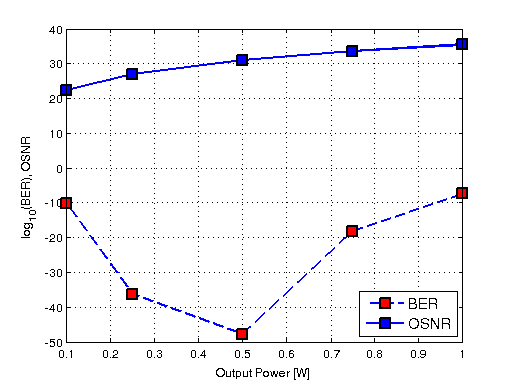
\includegraphics[width=11cm]{q1c1.png}\\
   \caption{BER and OSNR versus output power, fixed noise figure.}
   \label{q1c1}
\end{figure}
   
\begin{figure}[!ht]
   \centering
   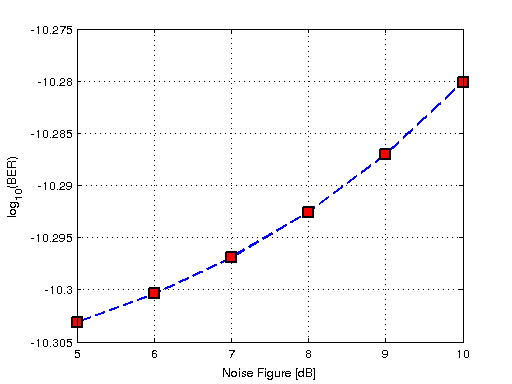
\includegraphics[width=11cm]{q1c2.png}\\
   \caption{BER versus noise figure, fixed output power.}
   \label{q1c2}
\end{figure}

\newpage
\begin{figure}[!ht]
   \centering
   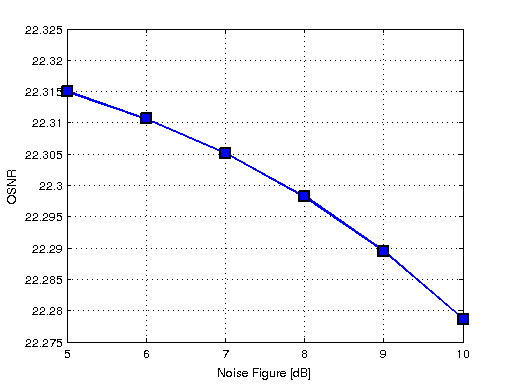
\includegraphics[width=11cm]{q1c3.png}\\
   \caption{OSNR versus noise figure, fixed output power.}
   \label{q1c3}
\end{figure}

We can observe that, when we vary the output power (with a fixed noise figure), the OSNR increases while the BER first decreases, and
then, for power values greater than 0.5 W, it starts increasing.
For the case in which we vary the noise figure (with fixed output power), instead, the BER monotonically increases, while the OSNR
monotonically decreases.


\newpage
%%%%%%%%%%%%%%%%%%%%%%%%%%%%%%%%%%%%%%%%%%%%%%%%%%%%%%%%%%%%%%%%%%%%%%%%%%%%%%%%%%%%%%%%%%%%%
\section*{6x10 Gbps Over 7500 Km}

Now we study a system with 64 channels at 10 Gb/s each. Three loop structures allow to achieve a distance of 7500 Km.
The fiber in the two loops has the following characteristics:
Dispersion $D=2 \cdot 10^{-6} \ [s/m^2]$ and dispersion slope $S=0.08 \cdot 10^{3} \ [s/m^3]$.
At each loop we have 10 dB of losses compensated by 10 dB of gain.

The fiber of the central link is a Single Mode Fiber (SMF) with tunable parameters. Its length is $\approx 58.8$ Km.


%%%%%%%%%%%%%%%%%%%%%%%%%%%%%%%%%%%%%%%%%%%%%%%%%%%%%%%%%%%%%%%%%%%%%%%%%%%%%%%%%%%%%%%%%%%%%
\subsection*{Question 2A}
Increasing the transmitted power we increase also the non-linear effects, so it is important to transmit
with the right quantity of power.
To find the optimal power value we start by running the simulation with the default parameters:\\
$D=-1.7 \cdot 10^{-5} \ [s/m^2]$, $S=80 \ [s/m^3]$ and $P=20 \ mW$.
In Figure \ref{q2_1} is shown the correspondent eye diagram.

\begin{figure}[!ht]
   \centering
   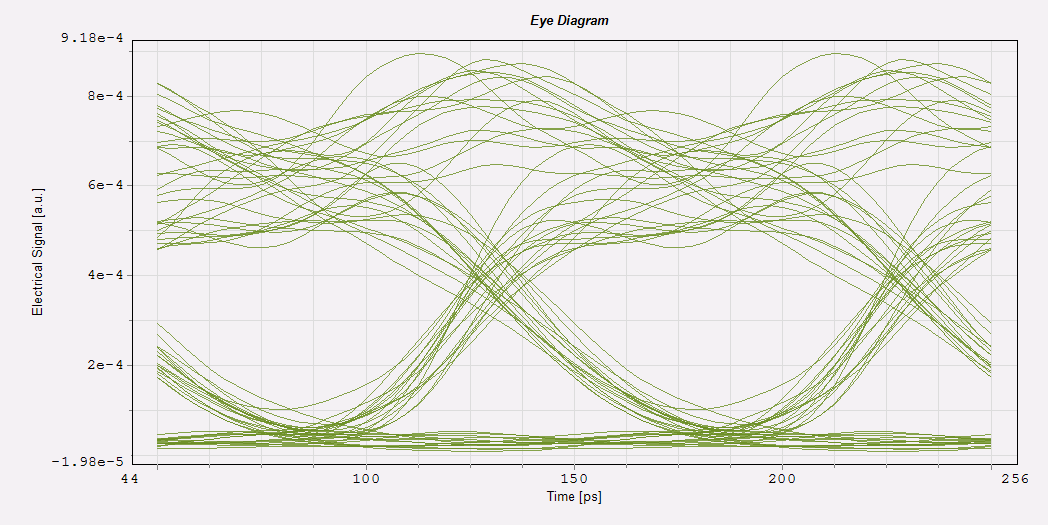
\includegraphics[width=12cm]{q2_1.png}\\
   \caption{Eye diagram $P=20 \ mW$.}
   \label{q2_1}
\end{figure}

We decrease the power and we set it to 10 mW: in Figure \ref{q2_2} is shown the eye diagram.
\begin{figure}[!ht]
   \centering
   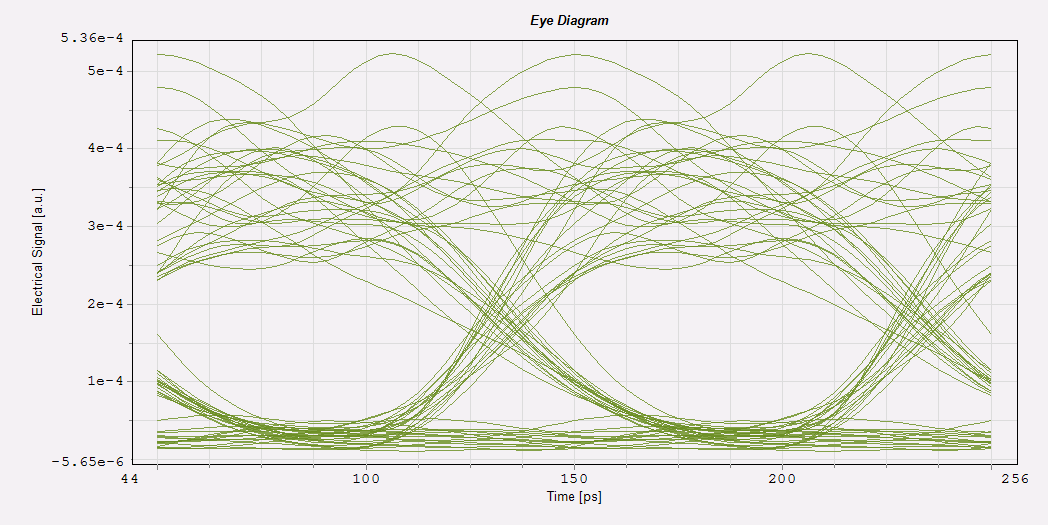
\includegraphics[width=12cm]{q2_2.png}\\
   \caption{Eye diagram $P=10 \ mW$.}
   \label{q2_2}
\end{figure}

Then we increase the power and we set it to 30 mW. In Figure \ref{q2_3} is shown the result.
\begin{figure}[!ht]
   \centering
   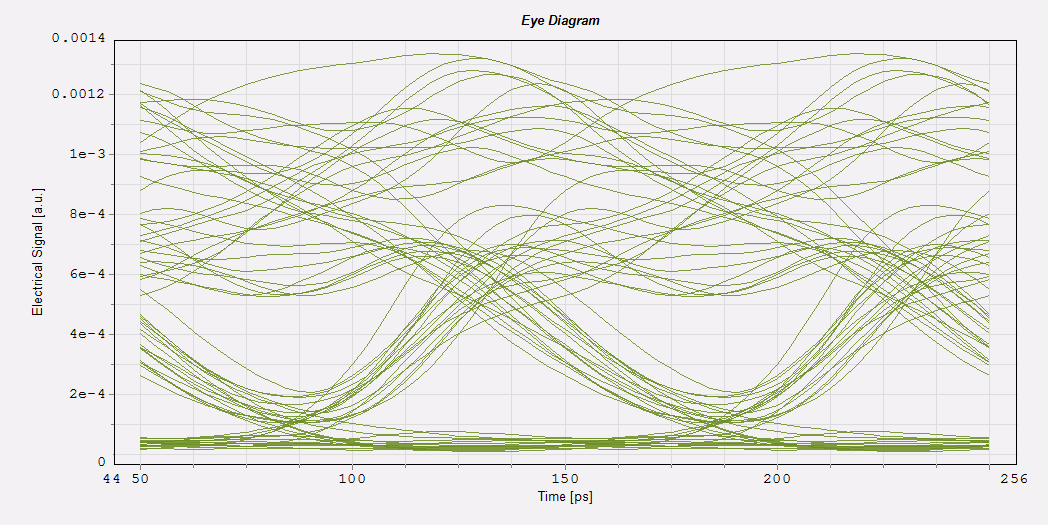
\includegraphics[width=12cm]{q2_3.png}\\
   \caption{Eye diagram $P=30 \ mW$.}
   \label{q2_3}
\end{figure}

We can observe that non-linearities degrade the signal.
By examining the obtained eye diagrams, we can conclude that the optimal power at the transmitter output is around 20 mW.


%%%%%%%%%%%%%%%%%%%%%%%%%%%%%%%%%%%%%%%%%%%%%%%%%%%%%%%%%%%%%%%%%%%%%%%%%%%%%%%%%%%%%%%%%%%%%
\subsection*{Question 2B}
A Dispersion Compensated Fiber (DCF) is needed to compensate the dispersion introduced and accumulated by the two loops.
In fact, the system is composed of two loops of 50 Km each. Each loop is repeated 5 times, so the total length of the loops
is 500 Km. The dispersion of the fiber used in the loops is $D=2 \cdot 10^{-6} \ [m/s^2]$.
The length of the fiber on the link in which we can compensate the dispersion is $L=10^3/17\approx 58.8 \ Km$, so to obtain the dispersion 
compensation value we apply the formula: $$ D_1 \cdot L_1 = - D_2 \cdot L_2$$
and so $$D_2=-\frac{D_1 \cdot L_1}{L_2}= -\frac{2 \cdot 10^{-6} \ [s/m^2] \cdot 500 \ [Km]}{58.8 \ [Km]}=-1.7 \cdot 10^{-5} \ [s/m^2]$$
that is exactly the default simulation value.
The dispersion slope allows to compensate the dispersion for different wavelength channels: otherwise, applying the same compensation
to all the channels, we would obtain a residual dispersion.
By repeating similar steps like in Question 2A, we can observe that the optimal dispersion slope is $S=80 \ [s/m^3]$, that is the default one.

\newpage
%%%%%%%%%%%%%%%%%%%%%%%%%%%%%%%%%%%%%%%%%%%%%%%%%%%%%%%%%%%%%%%%%%%%%%%%%%%%%%%%%%%%%%%%%%%%%
\section*{Multiplexing of Services}

Now we study how several services can be mixed in the same transmission system for applications in a metropolitan access network.
The system is composed of 40 channels at 2.5 Gb/s with 25 GHz spacing, and 10 channels at 10 Gb/s with 100 GHz spacing.
We work in the C band (1538-1554 nm).
The simulation values are the following:

\begin{itemize}
 \item Non linear index: $2.6 \cdot 10^{-20} $ [m$^2$/W]
 \item Length: $5 \cdot 10^{4}$ m
 \item Output power: $10^{-3}$ W
\end{itemize}


%%%%%%%%%%%%%%%%%%%%%%%%%%%%%%%%%%%%%%%%%%%%%%%%%%%%%%%%%%%%%%%%%%%%%%%%%%%%%%%%%%%%%%%%%%%%%
\subsection*{Question 3A}

According to the model, the wavelength band allocated to the 2.5 Gb/s channels goes from 1547 to 1554 nm, so in total it is
7 nm. The band for the 10 Gb/s channels goes from 1538 to 1545 nm, so in total it is 7 nm as well.
The wavelength corresponding to the first peak of the 2.5 Gb/s channels is at 1555.2 nm and the one of the last is at 1547.4 nm.
The difference is so $\approx 7.82$ nm.
For the 40 Gb/s channels, the first peak is at 1539.3 nm, while the last is at 1546.4 nm the difference is again $\approx 7.82$ nm.
The theoretical bandwidth is not the same as the one of the simulation: in fact we have to take into account that lasers and WDM filters
are not ideal devices.

%%%%%%%%%%%%%%%%%%%%%%%%%%%%%%%%%%%%%%%%%%%%%%%%%%%%%%%%%%%%%%%%%%%%%%%%%%%%%%%%%%%%%%%%%%%%%
\subsection*{Question 3B}

We increase the fiber length from 50 Km to 100 Km. In Figure \ref{q3b_1} and \ref{q3b_2} are shown the waveforms
for the 10 Gb/s and for the 40 Gb/s transmissions respectively.
As we can observe from the figures, the most degraded channels are the ones with higher rate, so the 40 Gb/s ones.


\begin{figure}[!ht]
   \centering
   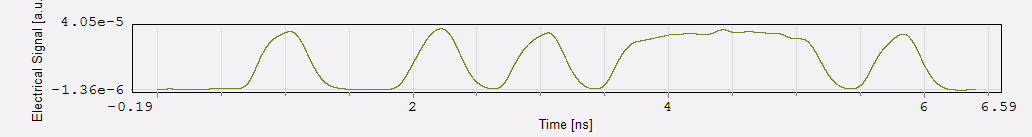
\includegraphics[width=12cm]{q3b_1.png}\\
   \caption{Waveform, 10 Gb/s.}
   \label{q3b_1}
\end{figure}


\begin{figure}[!ht]
   \centering
   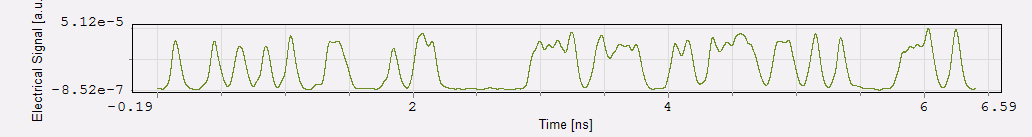
\includegraphics[width=12cm]{q3b_2.png}\\
   \caption{Waveform, 40 Gb/s.}
   \label{q3b_2}
\end{figure}


%%%%%%%%%%%%%%%%%%%%%%%%%%%%%%%%%%%%%%%%%%%%%%%%%%%%%%%%%%%%%%%%%%%%%%%%%%%%%%%%%%%%%%%%%%%%%
\subsection*{Question 3C}

In some cases it is possible to improve the maximum transmission distance by increasing the input power,
but it must be payed attention to the fact that, by increasing the power, also non-linear effects increase.
So there exists a trade-off between power and non linear effects, and consequently maximum
reachable distance.



%%%%%%%%%%%%%%%%%%%%%%%%%%%%%%%%%%%%%%%%%%%%%%%%%%%%%%%%%%%%%%%%%%%%%%%%%%%%%%%%%%%%%%%%%%%%%
\section*{Ring Routing}

We study now ring topologies. In particular we have an unidirectional ring created by using
point-to-point fiber segments between Add Drop Multiplexers (ADMs).
The ADMs are located in correspondence of nodes 1, 2 and 3.

%%%%%%%%%%%%%%%%%%%%%%%%%%%%%%%%%%%%%%%%%%%%%%%%%%%%%%%%%%%%%%%%%%%%%%%%%%%%%%%%%%%%%%%%%%%%%
\subsection*{Question 4A}
The signal is routed from the entry points to the exits by the means of the multiplexers.

%%%%%%%%%%%%%%%%%%%%%%%%%%%%%%%%%%%%%%%%%%%%%%%%%%%%%%%%%%%%%%%%%%%%%%%%%%%%%%%%%%%%%%%%%%%%%
\subsection*{Question 4B}
The communication between nodes is unidirectional.

%%%%%%%%%%%%%%%%%%%%%%%%%%%%%%%%%%%%%%%%%%%%%%%%%%%%%%%%%%%%%%%%%%%%%%%%%%%%%%%%%%%%%%%%%%%%%
\subsection*{Question 4C}
In each fiber segment there are three wavelengths circulating. At each node one wavelength is
added and one is dropped. In Figure \ref{qc} is shown the result.

\begin{figure}[!ht]
   \centering
   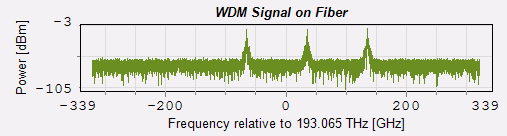
\includegraphics[width=12cm]{qc.png}\\
   \caption{Optical spectrum.}
   \label{qc}
\end{figure}

%%%%%%%%%%%%%%%%%%%%%%%%%%%%%%%%%%%%%%%%%%%%%%%%%%%%%%%%%%%%%%%%%%%%%%%%%%%%%%%%%%%%%%%%%%%%%
\subsection*{Question 4D}
By increasing the fiber lengths from 80 Km to 120 Km, the outputs are degraded.
In Figure \ref{q4d_1} is shown the power waveform at the output of node 2, for a length of 80 Km,
while in Figure \ref{q4d_2} is shown the same result for a length of 120 Km.

\begin{figure}[!ht]
   \centering
   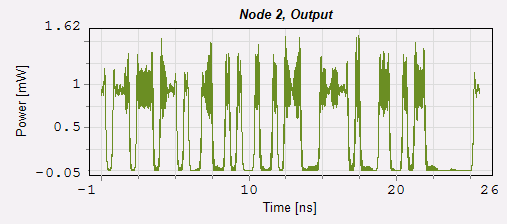
\includegraphics[width=12cm]{q4d_1.png}\\
   \caption{Output power, 80 Km.}
   \label{q4d_1}
\end{figure}


\begin{figure}[!ht]
   \centering
   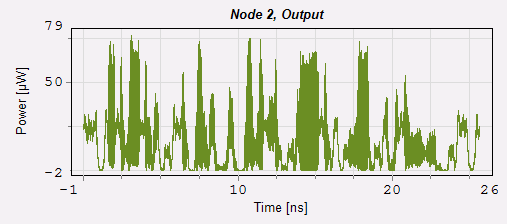
\includegraphics[width=12cm]{q4d_2.png}\\
   \caption{Output power, 120 Km.}
   \label{q4d_2}
\end{figure}


\newpage
%%%%%%%%%%%%%%%%%%%%%%%%%%%%%%%%%%%%%%%%%%%%%%%%%%%%%%%%%%%%%%%%%%%%%%%%%%%%%%%%%%%%%%%%%%%%%
\section*{3x Ring with OXC $\&$ ADM}
The schematic consists of three rings linked by Add Drop Multiplexers (ADMs) and Optical Cross Connects (OXCs).
The ADMs are located in correspondence of the lasers to link them with the fibers, and between ring 1 and ring 2, to connect them.

%%%%%%%%%%%%%%%%%%%%%%%%%%%%%%%%%%%%%%%%%%%%%%%%%%%%%%%%%%%%%%%%%%%%%%%%%%%%%%%%%%%%%%%%%%%%%
\subsection*{Question 5A}
In each ADM that connects ring 1 with ring 2 are extracted three wavelengths.
In the others is extract one wavelength.

%%%%%%%%%%%%%%%%%%%%%%%%%%%%%%%%%%%%%%%%%%%%%%%%%%%%%%%%%%%%%%%%%%%%%%%%%%%%%%%%%%%%%%%%%%%%%
\subsection*{Question 5B}
Between ring 1 and ring 2 can be exchanged 3 channels.
In Figure \ref{q5b} is shown the result.

\begin{figure}[!ht]
   \centering
   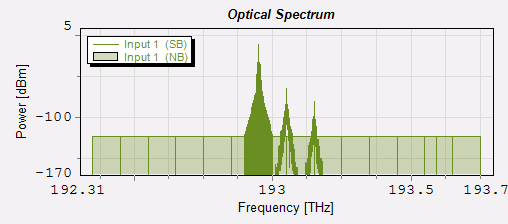
\includegraphics[width=12cm]{q5b.png}\\
   \caption{Optical spectrum.}
   \label{q5b}
\end{figure}

%%%%%%%%%%%%%%%%%%%%%%%%%%%%%%%%%%%%%%%%%%%%%%%%%%%%%%%%%%%%%%%%%%%%%%%%%%%%%%%%%%%%%%%%%%%%%
\subsection*{Question 5C}
Between ring 3 and ring 2 can be exchanged 4 channels.
In Figure \ref{q5c} is shown the result.

\begin{figure}[!ht]
   \centering
   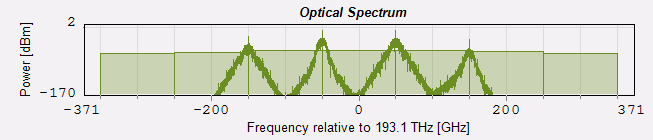
\includegraphics[width=12cm]{q5c.png}\\
   \caption{Optical spectrum.}
   \label{q5c}
\end{figure}

%%%%%%%%%%%%%%%%%%%%%%%%%%%%%%%%%%%%%%%%%%%%%%%%%%%%%%%%%%%%%%%%%%%%%%%%%%%%%%%%%%%%%%%%%%%%%
\subsection*{Question 5D}
The signal is routed from the entry points to the exits by the means of the multiplexers.

%%%%%%%%%%%%%%%%%%%%%%%%%%%%%%%%%%%%%%%%%%%%%%%%%%%%%%%%%%%%%%%%%%%%%%%%%%%%%%%%%%%%%%%%%%%%%
\subsection*{Question 5E}
We set the parametes Fiber In Rings Active and Long Haul Link Active to OFF, to see only the effect of the filters.
The dispersions of the pre-compensation and of the post-compensation are initially set to $D_{pre}=D_{post}=5 \cdot 10^{-1}$.
We vary the amount of the dispersions and we measure the BER of the output signal in ring 3: in Table \ref{tab3} are reported the results.

\begin{table}[ht!]
  \begin{center}
    \begin{tabular}{|c|c|c|}
      \specialrule{.1em}{.05em}{.05em}
	D$_{pre}$ & D$_{post}$ & BER\\
	\hline
	$5 \cdot 10^{-1}$ & $5 \cdot 10^{-1}$ & $9.59 \cdot 10^{-43}$\\
	\hline
	$1 \cdot 10^{-1}$ & $5 \cdot 10^{-1}$ & $3.16 \cdot 10^{-6}$\\
	\hline
	$5 \cdot 10^{-1}$ & $1 \cdot 10^{-1}$ & $3.16 \cdot 10^{-6}$\\
	\hline
	$1 \cdot 10^{-1}$ & $9 \cdot 10^{-1}$ & $9.59 \cdot 10^{-43}$\\
	\hline
	$9 \cdot 10^{-1}$ & $1 \cdot 10^{-1}$ & $9.59 \cdot 10^{-43}$\\
	
      \specialrule{.1em}{.05em}{.05em}
    \end{tabular}
  \end{center}
\caption{Dispersions comparison.}
\label{tab3}
\end{table}

We can observe that, when the total dispersion is equal to 1, the obtained BER is the same.


\newpage
%%%%%%%%%%%%%%%%%%%%%%%%%%%%%%%%%%%%%%%%%%%%%%%%%%%%%%%%%%%%%%%%%%%%%%%%%%%%%%%%%%%%%%%%%%%%%
\section*{Optical Switching}
We study the operation of an Optical Cross Connect (OXC).

%%%%%%%%%%%%%%%%%%%%%%%%%%%%%%%%%%%%%%%%%%%%%%%%%%%%%%%%%%%%%%%%%%%%%%%%%%%%%%%%%%%%%%%%%%%%%
\subsection*{Question 6A}
The function of the demultiplexers is to separate different wavelength channels coming from one fiber. In this case we demultiplex four channels,
that is, from one fiber that contains four wavelength signals, we extract each signal on a separate fiber.
The multiplexers, instead, have the function to merge different wavelength channels (coming from different fibers)
into a single fiber.

%%%%%%%%%%%%%%%%%%%%%%%%%%%%%%%%%%%%%%%%%%%%%%%%%%%%%%%%%%%%%%%%%%%%%%%%%%%%%%%%%%%%%%%%%%%%%
\subsection*{Question 6B}
The switch fabric is made of 4 switches. Each of these switches is composed of 6 switching blocks, so the total number of switches is 24.

%%%%%%%%%%%%%%%%%%%%%%%%%%%%%%%%%%%%%%%%%%%%%%%%%%%%%%%%%%%%%%%%%%%%%%%%%%%%%%%%%%%%%%%%%%%%%
\subsection*{Question 6C}
We do need frequency converters as the system allows to switch two frequency channels from one input to
any frequency to the other output. To do this we need to convert the frequency of the channels into the desired one.


\newpage
%%%%%%%%%%%%%%%%%%%%%%%%%%%%%%%%%%%%%%%%%%%%%%%%%%%%%%%%%%%%%%%%%%%%%%%%%%%%%%%%%%%%%%%%%%%%%
\section*{Optical Packet Network}

%%%%%%%%%%%%%%%%%%%%%%%%%%%%%%%%%%%%%%%%%%%%%%%%%%%%%%%%%%%%%%%%%%%%%%%%%%%%%%%%%%%%%%%%%%%%%
\subsection*{Question 7A}
The port is selected by looking at 2 bits at the beginning of the header.
In Figure \ref{q7a} is reported the sequence of header values for the 8 packets, so from that we can deduce the sequence of
selected ports, that is: $$3 \ - 1 \ - 0 \ - 0 \ - 0 \ - 2 \ - 3 \ - 0$$

\begin{figure}[!ht]
   \centering
   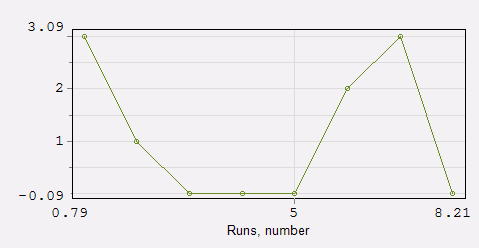
\includegraphics[width=12cm]{q7a.png}\\
   \caption{Header values.}
   \label{q7a}
\end{figure}

%%%%%%%%%%%%%%%%%%%%%%%%%%%%%%%%%%%%%%%%%%%%%%%%%%%%%%%%%%%%%%%%%%%%%%%%%%%%%%%%%%%%%%%%%%%%%
\subsection*{Question 7B}
If the packet arrives at the switch fabric before the header is processed it cannot be correctly routed,
as the destination port is unknown.

%%%%%%%%%%%%%%%%%%%%%%%%%%%%%%%%%%%%%%%%%%%%%%%%%%%%%%%%%%%%%%%%%%%%%%%%%%%%%%%%%%%%%%%%%%%%%
\subsection*{Question 7C}
The problem can be solved by using an optical buffer to delay the incoming packets.


\newpage
%%%%%%%%%%%%%%%%%%%%%%%%%%%%%%%%%%%%%%%%%%%%%%%%%%%%%%%%%%%%%%%%%%%%%%%%%%%%%%%%%%%%%%%%%%%%%
\section*{OADM Protection Switching 1}
This setup uses a unidirectional ring that has a second fiber used only for protection.

%%%%%%%%%%%%%%%%%%%%%%%%%%%%%%%%%%%%%%%%%%%%%%%%%%%%%%%%%%%%%%%%%%%%%%%%%%%%%%%%%%%%%%%%%%%%%
\subsection*{Question 8A}
Before the failure there were no channels occupied in the protection fiber. After the failure 3 channels were occupied.
In Figure \ref{q8a} it is possible to see the results.

\begin{figure}[!ht]
   \centering
   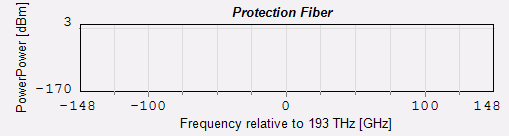
\includegraphics[width=12cm]{q8a1.png}\\
   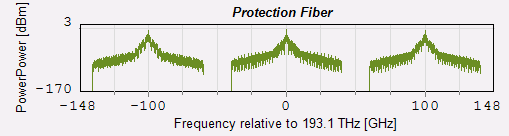
\includegraphics[width=12cm]{q8a2.png}\\
   \caption{Channels occupation before (above) and after (bottom) the failure.}
   \label{q8a}
\end{figure}

%%%%%%%%%%%%%%%%%%%%%%%%%%%%%%%%%%%%%%%%%%%%%%%%%%%%%%%%%%%%%%%%%%%%%%%%%%%%%%%%%%%%%%%%%%%%%
\subsection*{Question 8B}
Before the failure, in the working fiber behind the fiber cut, there were occupied 2 channels.
After the failure zero channels were occupied.
In Figure \ref{q8b} it is possible to see the results.

\begin{figure}[!ht]
   \centering
   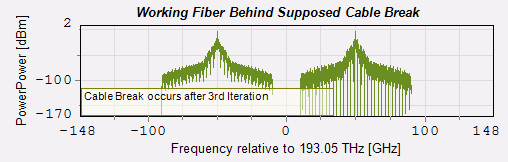
\includegraphics[width=12cm]{q8b1.png}\\
   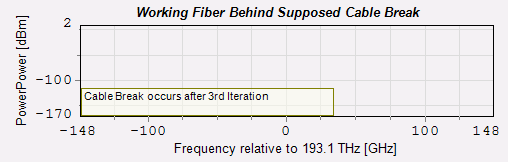
\includegraphics[width=12cm]{q8b2.png}\\
   \caption{Channels occupation before (above) and after (bottom) the failure.}
   \label{q8b}
\end{figure}

%%%%%%%%%%%%%%%%%%%%%%%%%%%%%%%%%%%%%%%%%%%%%%%%%%%%%%%%%%%%%%%%%%%%%%%%%%%%%%%%%%%%%%%%%%%%%
\subsection*{Question 8C}
In the working fiber away from the cut, before the failure, it was occupied one channel.
After the failure one channel was occupied.
In Figure \ref{q8c} it is possible to see the results.

\begin{figure}[!ht]
   \centering
   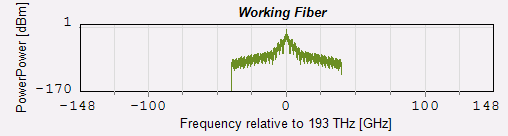
\includegraphics[width=12cm]{q8c1.png}\\
   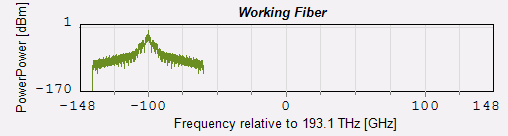
\includegraphics[width=12cm]{q8c2.png}\\
   \caption{Channels occupation before (above) and after (bottom) the failure.}
   \label{q8c}
\end{figure}

%%%%%%%%%%%%%%%%%%%%%%%%%%%%%%%%%%%%%%%%%%%%%%%%%%%%%%%%%%%%%%%%%%%%%%%%%%%%%%%%%%%%%%%%%%%%%
\subsection*{Question 8D}
During a failure, the signal is protected by a re-routing from the working fiber to the protection fiber.



%%%%%%%%%%%%%%%%%%%%%%%%%%%%%%%%%%%%%%%%%%%%%%%%%%%%%%%%%%%%%%%%%%%%%%%%%%%%%%%%%%%%%%%%%%%%%
\section*{OADM Protection Switching 2}
This setup implements a bidirectional ring that uses both fibers at half capacity.

%%%%%%%%%%%%%%%%%%%%%%%%%%%%%%%%%%%%%%%%%%%%%%%%%%%%%%%%%%%%%%%%%%%%%%%%%%%%%%%%%%%%%%%%%%%%%
\subsection*{Question 9A}
In each fiber, before the failure were occupied 4 channels. It is possible to see the results in\\ Figure \ref{q9a}.

\begin{figure}[!ht]
   \centering
   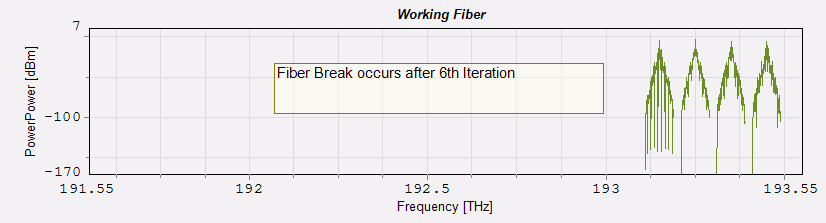
\includegraphics[width=12cm]{q9a1.png}\\
   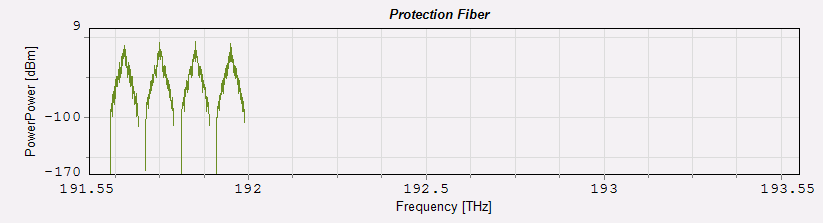
\includegraphics[width=12cm]{q9a2.png}\\
   \caption{Channels occupation before the failure.}
   \label{q9a}
\end{figure}

%%%%%%%%%%%%%%%%%%%%%%%%%%%%%%%%%%%%%%%%%%%%%%%%%%%%%%%%%%%%%%%%%%%%%%%%%%%%%%%%%%%%%%%%%%%%%
\subsection*{Question 9B}
After the failure, in each fiber were occupied 8 channels. It is possible to see the results in\\ Figure \ref{q9b}.

\begin{figure}[!ht]
   \centering
   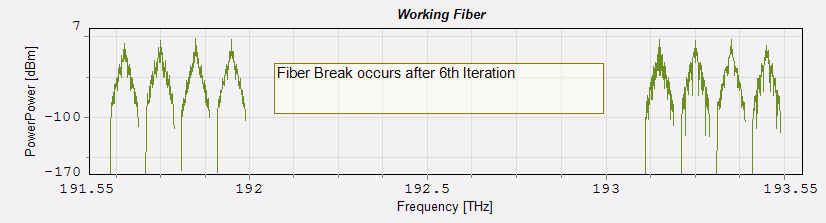
\includegraphics[width=12cm]{q9a3.png}\\
   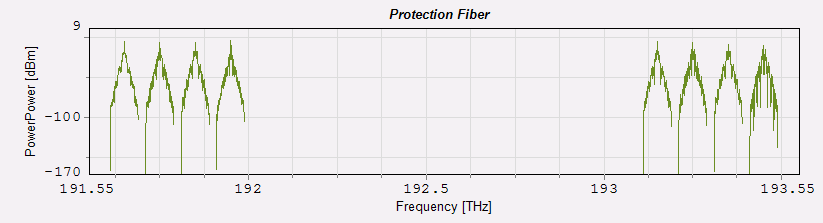
\includegraphics[width=12cm]{q9a4.png}\\
   \caption{Channels occupation after the failure.}
   \label{q9b}
\end{figure}

%%%%%%%%%%%%%%%%%%%%%%%%%%%%%%%%%%%%%%%%%%%%%%%%%%%%%%%%%%%%%%%%%%%%%%%%%%%%%%%%%%%%%%%%%%%%%
\subsection*{Question 9C}
During a failure the communication is switched from bidirectional to unidirectional and
each fiber transports double load respect to the case of normal working conditions.





\end{document}